\chapter{Pilot Validation Study}
\label{ch:evaluation}

This chapter presents the pilot validation study used to evaluate whether HRIStudio improves accessibility and reproducibility in WoZ-based HRI research. It defines the research questions, study design, task, apparatus, procedure, and measurement instruments.

\section{Research Questions}

The validation study targets the two problems established in Chapter~\ref{ch:background}. The first is the \emph{Accessibility Problem}: existing tools require substantial programming expertise, which prevents domain experts from conducting independent HRI studies. The second is the \emph{Reproducibility Problem}: without structured logging and protocol enforcement, experiment execution varies across participants and wizards in ways that are difficult to detect or control after the fact.

These problems give rise to two research questions. The first is whether HRIStudio enables domain experts without prior robotics experience to successfully implement a robot interaction from a written specification. The second is whether HRIStudio produces more reliable execution of that interaction compared to standard practice.

I hypothesized that HRIStudio would improve both accessibility and reproducibility compared to Choregraphe: wizards using HRIStudio would more completely and correctly implement the written specification, and their designs would execute more reliably during the trial.

\section{Study Design}

I used what Bartneck et al.~\cite{Bartneck2024} call a \emph{between-subjects design}, in which each participant is assigned to only one condition. To ensure that programming experience was balanced across conditions, I stratified assignment by self-reported programming background: each wizard was first classified as having \emph{None}, \emph{Moderate}, or \emph{Extensive} programming experience, and then randomly assigned within that stratum to HRIStudio or Choregraphe. This produced a design in which each condition contained exactly one wizard at each experience level, reducing the risk that tool effects would be confused with differences in programming experience. Both groups received the same task, the same time allocation, and a similar training structure. Because each wizard used only one tool, the design also avoided carryover effects from prior exposure to the other condition.

\section{Participants}

\textbf{Wizards.} A primary claim of HRIStudio is that it lowers the technical barrier for domain experts who are not programmers; testing this claim with its intended user population was therefore a primary goal of participant recruitment. I recruited six Bucknell University faculty members drawn from across departments to serve as wizards, deliberately targeting both ends of the programming experience spectrum: those with substantial programming backgrounds as well as those who described themselves as non-programmers or having minimal coding experience. Drawing wizards from outside computer science allows the data to speak to whether that claim holds for the intended user population.

The key inclusion criterion for all wizards was no prior experience with either the NAO robot or Choregraphe software specifically. This controls for tool familiarity so that performance differences reflect the tools themselves rather than prior exposure. I recruited wizards through direct email, and participation was framed as a voluntary software evaluation unrelated to any professional obligations.

\textbf{Sample size rationale.} I chose to recruit six wizard participants ($N = 6$), believing that this sample size is appropriate for a pilot validation study whose goal is directional evidence and failure-mode identification rather than effect-size estimation for a broad population. This scale is consistent with pilot and feasibility studies in HRI, where small $N$ designs are common in early-stage tool validation~\cite{HoffmanZhao2021}. Findings should be interpreted as preliminary evidence and directional indicators rather than as conclusive substantiation of any claims.

\section{Task}

The task chosen was to have a robot tell a story to a human subject and later evaluate if that subject could recall a specific detail.

Both wizard groups received the same written task specification: the \emph{Interactive Storyteller} scenario. The specification described a robot that introduces an astronaut named Kai, narrates her discovery of a red rock on Mars, asks a recall question, and delivers a response according to the answer given. The full specification, including exact robot speech, required gestures, and branching logic, is reproduced in Appendix~\ref{app:blank_templates}. This scenario is representative of HRI tasks in which a robot conveys information to a human subject; one might, for example, measure whether a robot or human storyteller produces better recall in subjects.

This scenario was chosen because it requires several distinct capabilities: speech actions, gesture coordination, conditional branching, and a defined conclusion. In both conditions, wizards had to translate the same written protocol into an executable interaction script, including action ordering, branching logic, and timing decisions. In Choregraphe, that meant assembling and connecting behavior nodes in a finite state machine. In HRIStudio, it meant building a sequential action timeline with conditional branches. This makes the task a direct comparison of how each tool supports coding the robot behavior required by the same protocol.

\section{Robot Platform and Software Apparatus}

Both conditions used the same NAO humanoid robot (Figure~\ref{fig:nao6-photo}), a platform approximately 0.58 meters tall capable of speech synthesis, animated gestures, and head movement. Using the same hardware ensured that any differences in execution quality were attributable to the software, not the robot.


\begin{figure}[htbp]
\centering
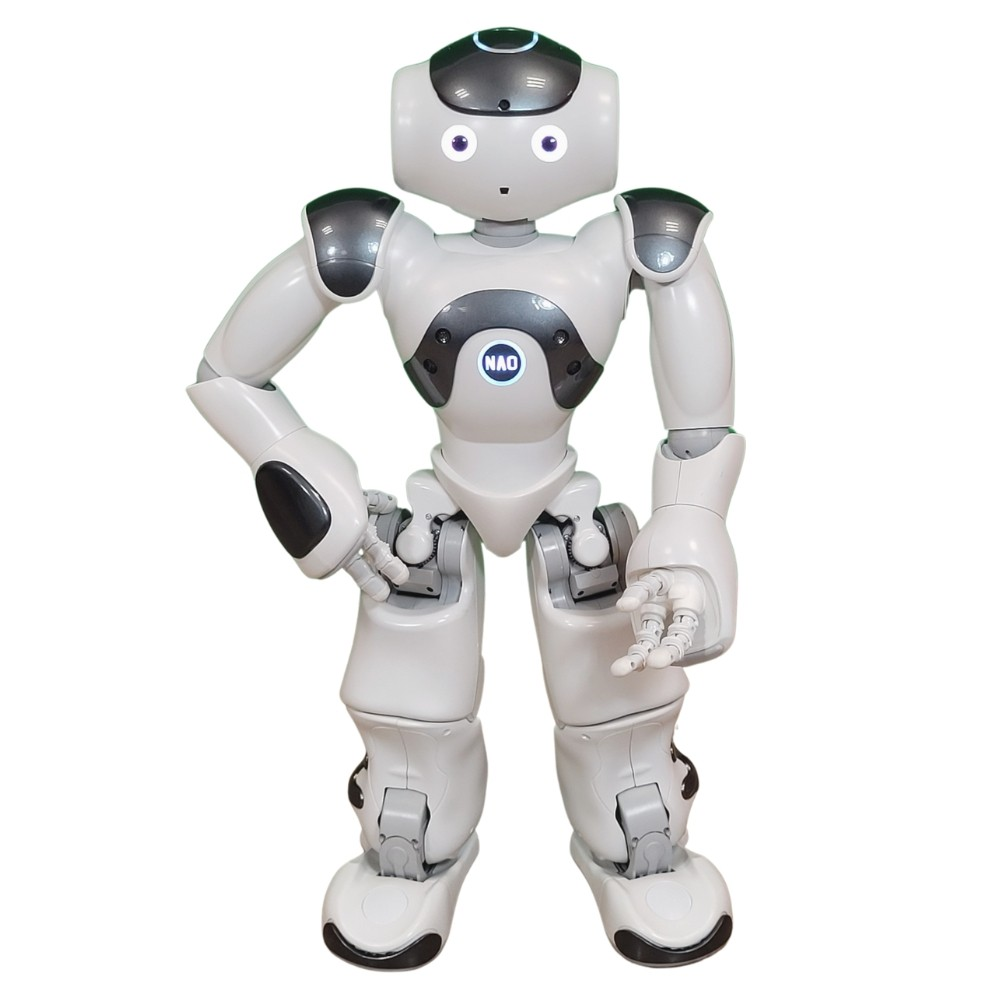
\includegraphics[width=0.45\textwidth]{images/nao6.jpg}
\caption{The NAO6 humanoid robot used in both conditions of the pilot study.}
\label{fig:nao6-photo}
\end{figure}


The control condition used Choregraphe \cite{Pot2009}, a proprietary visual programming tool developed by Aldebaran Robotics and the standard software for NAO programming. Choregraphe organizes behavior as a finite state machine: nodes represent states and edges represent transitions triggered by conditions or timers.

The experimental condition used HRIStudio, described in Chapter~\ref{ch:implementation}. HRIStudio organizes behavior as a sequential action timeline with support for conditional branches. Unlike Choregraphe, it abstracts robot-specific commands through plugin files, though for this study both tools controlled the same NAO platform.

Figure~\ref{fig:design-tool-compare} places the two design environments side by side. On the left, Choregraphe's behavior-box canvas (Figure~\ref{fig:choregraphe-ui}) lets the wizard wire nodes and transitions in a finite-state-machine layout. On the right, HRIStudio's experiment designer (Figure~\ref{fig:hristudio-designer}) presents the same protocol as a vertical action timeline with dedicated blocks for speech, gesture, and conditional branching.

\begin{figure}[htbp]
\centering
\begin{minipage}[t]{0.48\textwidth}
\centering
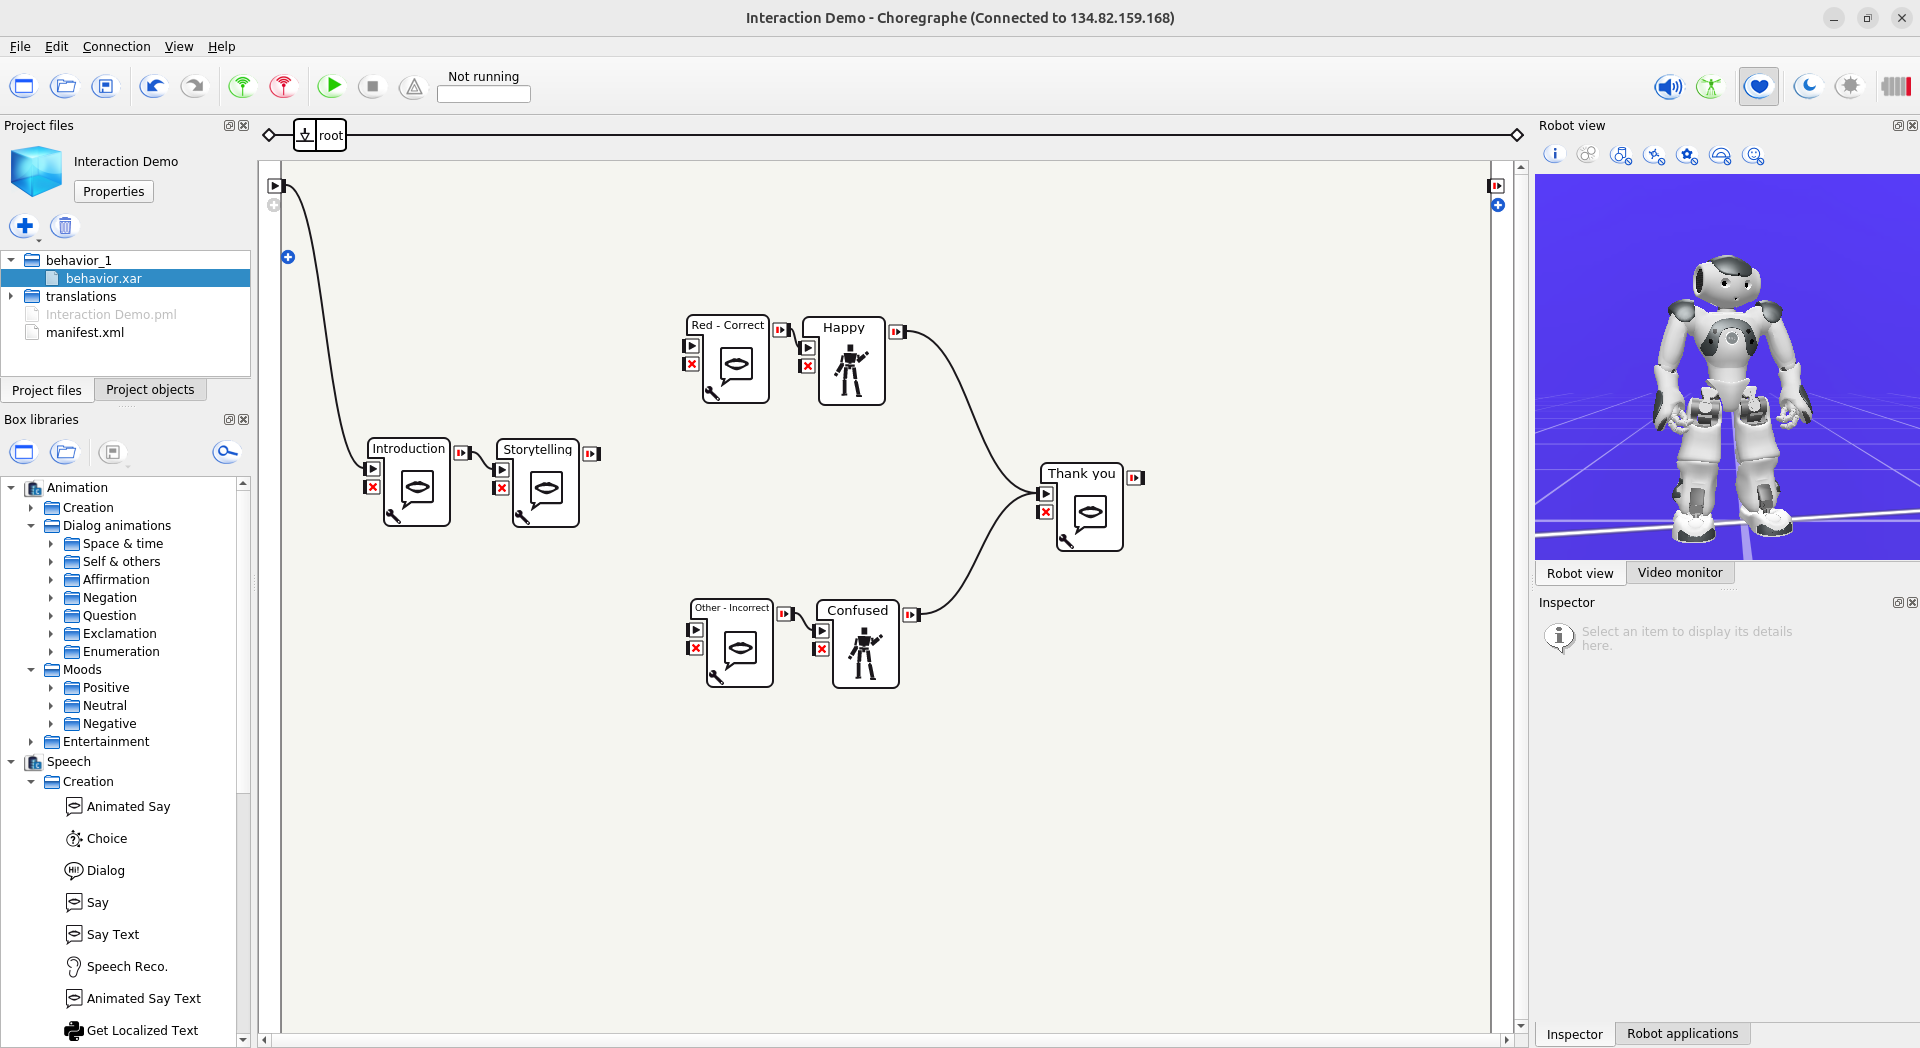
\includegraphics[width=\textwidth]{assets/choregraphe.png}
\subcaption{Choregraphe: behavior-box canvas with nodes and transitions.}
\label{fig:choregraphe-ui}
\end{minipage}\hfill
\begin{minipage}[t]{0.48\textwidth}
\centering
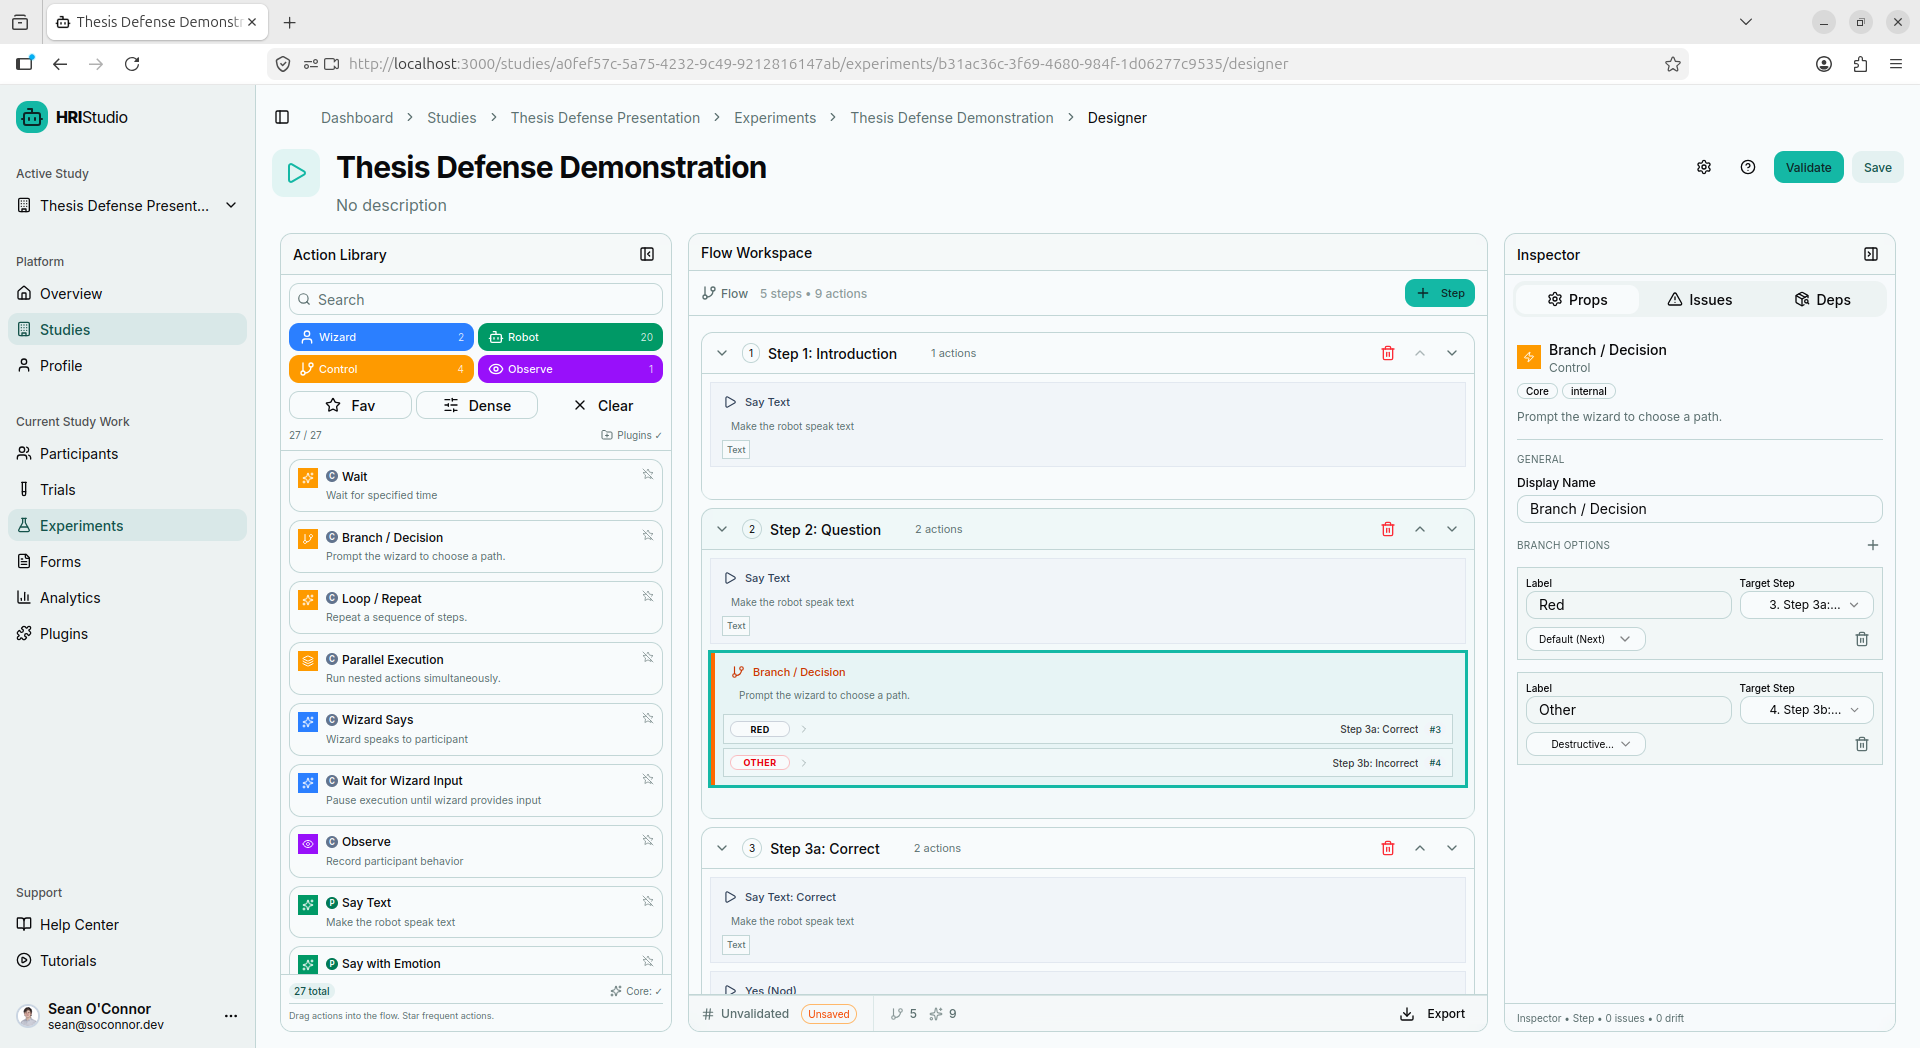
\includegraphics[width=\textwidth]{assets/experiment-designer.png}
\subcaption{HRIStudio: vertical action timeline with structured step and action blocks.}
\label{fig:hristudio-designer}
\end{minipage}
\caption{The two design environments compared. Each wizard used one of these tools to implement the Interactive Storyteller specification.}
\label{fig:design-tool-compare}
\end{figure}

\section{Procedure}

Each wizard completed a single 60-minute session structured in four phases.

\subsection{Phase 1: Training (15 minutes)}

I opened each session with a standardized tutorial tailored to the wizard's assigned tool. The tutorial covered how to create speech actions, specify gestures, define conditional branches, and save the completed design. Training was intentionally allocated 15 minutes to allow enough time for wizards to ask clarifying questions about the tool before the design challenge began, while still simulating first encounter with a new tool without extensive onboarding. I answered clarification questions during this phase but did not offer hints about the design challenge.

\subsection{Phase 2: Design Challenge (30 minutes)}

The wizard received the specification and had 30 minutes to implement it using their assigned tool. Using a structured observer data sheet (found in Appendix~\ref{app:blank_templates}), I logged every instance in which I provided assistance to the wizard, categorizing each by type: \emph{tool-operation} (T), \emph{task clarification} (C), \emph{hardware or technical} (H), or \emph{general} (G). For each tool-operation intervention, I also recorded which rubric item it pertained to. If the wizard declared completion before the time limit, the remaining time was used to review and refine the design.

\subsection{Phase 3: Live Trial (10 minutes)}

After the design phase, the wizard ran their completed program to execute the designed interaction on the robot. I continued logging any researcher interventions during the trial using the same type categories, noting the relevant ERS rubric item for any tool-operation intervention.

\subsection{Phase 4: Debrief (5 minutes)}

Following the trial, the wizard completed the System Usability Scale survey (found in Appendix~\ref{app:blank_templates}). The DFS and ERS were scored during and immediately after the session using live observation and the Observer Data Sheet.

\section{Measures}
\label{sec:measures}

The study collected five measures, two primary and three supplementary, operationalized through five instruments. They are described as follows.

\subsection{Design Fidelity Score}

I define the Design Fidelity Score (DFS) as a measure of how completely and correctly the wizard implemented the specification. I evaluated the exported project file against nine weighted criteria grouped into three categories: speech actions, gestures and actions, and control flow and logic. Each criterion is scored as present, correct, and independently achieved.

The DFS rubric includes an \emph{Assisted} column. For each rubric item, I marked a T if I provided a tool-operation intervention specifically for that item during the design phase (for example, if I explained how to add a gesture node or how to wire a conditional branch). T marks are recorded and reported separately alongside the DFS score; they do not affect the Points total. This preserves the DFS as a clean measure of design fidelity while providing a parallel record of where tool-specific assistance was needed. General interventions (task clarification, hardware issues, or momentary forgetfulness) are not marked T, because those categories of difficulty are independent of the tool under evaluation.

DFS is motivated by a gap identified by Riek~\cite{Riek2012}, whose systematic review of 54 published WoZ studies found that only 11\% constrained wizard behavior and fewer than 6\% described wizard training procedures. Porfirio et al.~\cite{Porfirio2023} similarly argued that formal, verifiable behavior specifications are a prerequisite for reproducible HRI. The DFS applies these recommendations as a weighted rubric scored against the exported project file. The complete rubric is reproduced in Appendix~\ref{app:blank_templates}. This measure addresses the question: did the tool allow a wizard to independently produce a correct design?

\subsection{Execution Reliability Score}

I define the Execution Reliability Score (ERS) as a measure of whether the designed interaction executed as intended during the live trial. I scored the ERS live and immediately after the session, using the Observer Data Sheet and the wizard's exported project file. Evaluation criteria included whether the robot delivered the correct speech at each step, whether gestures executed and synchronized with speech, whether the conditional branch was present in the design and executed during the trial, and whether any errors, disconnections, or hangs occurred.

The ERS rubric applies the same \emph{Assisted} modifier as the DFS, extended to the trial phase. Any tool-operation intervention I provided during the trial (for example, explaining to the wizard how to launch or advance their program) caps the affected ERS item at half points. This is scored separately from design-phase interventions: a wizard who needed help only during design can still achieve a full ERS score if the trial runs without assistance, and vice versa. The rubric records whether the trial reached its conclusion step. I additionally note whether any branch resolved through programmed conditional logic or through manual intervention by the wizard during execution.

This measure responds directly to Riek's~\cite{Riek2012} finding that only 3.7\% of published WoZ studies reported any measure of wizard error, making it nearly impossible to determine whether execution matched design intent~\cite{OConnor2024, OConnor2025}. The complete rubric is reproduced in Appendix~\ref{app:blank_templates}. This measure addresses the question: did the design translate reliably into execution without researcher support?

\subsection{System Usability Scale}

The System Usability Scale (SUS) is a validated 10-item questionnaire measuring perceived usability, created by Brooke~\cite{Brooke1996}. Wizards completed the SUS after the debrief phase. Scores range from 0 to 100, with higher scores indicating better perceived usability. The full questionnaire is reproduced in Appendix~\ref{app:blank_templates}.

\subsection{Intervention Log and Session Timing}

During each session, I maintained a structured intervention log on the observer data sheet, recording the timestamp, type code, affected rubric item number, and a brief description for every instance in which I assisted the wizard. The four intervention type codes are:

\begin{description}
    \item[T (tool-operation).] I explained how to operate a specific feature of the assigned software tool.
    \item[C (task clarification).] I clarified the written specification or an aspect of the task design.
    \item[H (hardware or technical).] I addressed a robot connection issue or other technical problem outside the wizard's control.
    \item[G (general).] Brief assistance not attributable to the tool or the task, such as momentary forgetfulness.
\end{description}

Only T-type interventions affect rubric scoring; the others are recorded to provide context for interpreting session flow and wizard experience. I also recorded the actual duration of each session phase and the time at which the wizard completed or abandoned the design, providing supplementary evidence about tool accessibility beyond the DFS score itself.

\section{Measurement Instruments}

The five measures are designed to work together. The DFS and ERS address separate phases of the session: DFS captures what was designed, and ERS captures whether that design translated faithfully into execution. Taken together, they make it possible to distinguish a wizard who implemented the specification correctly but whose design failed during the trial from one whose design was incomplete but executed without researcher assistance. The SUS grounds both scores in the wizard's subjective experience of the tool. The intervention log and session timing are supplementary: they do not directly answer the research questions but provide context for interpreting the primary scores, particularly for understanding whether help requests concerned the tool itself or the task.

Table~\ref{tbl:measurement_instruments} summarizes the five instruments, when they were collected, and which research question each addresses.

\begin{table}[htbp]
\centering
\footnotesize
\begin{tabular}{|p{3.0cm}|p{4.4cm}|p{2.4cm}|p{2.8cm}|}
\hline
\textbf{Instrument} & \textbf{What it captures} & \textbf{When collected} & \textbf{Research question} \\
\hline
Design Fidelity Score (DFS) & Completeness and correctness of the wizard's implementation; caps items where tool-operation assistance was given & Post-session file review & Accessibility \\
\hline
Execution Reliability Score (ERS) & Whether the interaction executed as designed during the trial; caps items where trial-phase tool assistance occurred & Live and post-trial (ODS) & Reproducibility \\
\hline
System Usability Scale (SUS) & Wizard's perceived usability of the assigned tool & Debrief phase & User experience \\
\hline
Intervention Log & Timestamped record of all researcher assistance by type (T/C/H/G) and affected rubric item & Throughout session & Supplementary \\
\hline
Session Timing & Actual duration of each phase; time to design completion & Throughout session & Supplementary \\
\hline
\end{tabular}
\caption{Measurement instruments used in the pilot validation study.}
\label{tbl:measurement_instruments}
\end{table}

\section{Chapter Summary}

This chapter described the structure of a pilot between-subjects study I designed to test whether the design principles formalized in Chapters~\ref{ch:design} and~\ref{ch:implementation} produce measurably different outcomes from existing practice. Six wizard participants ($N = 6$), drawn from across departments and spanning the programming experience spectrum, each designed and ran the Interactive Storyteller task on a NAO robot using either HRIStudio or Choregraphe. Each 60-minute session was structured in four phases: a 15-minute standardized tutorial, a 30-minute design challenge, a 10-minute live trial, and a 5-minute debrief. I measured design fidelity (DFS) and execution reliability (ERS) against the written specification, applying a per-item scoring modifier that caps any rubric criterion for which tool-operation assistance was given. I also collected perceived usability via the SUS, a structured intervention log categorizing all researcher assistance by type, and session phase timings. Chapter~\ref{ch:results} presents the results.
